\chapter{Mapping. Spheroidal coordinates}

We have seen at the end of the previous chapter that we can work with
2D problems combining {\tt diff\_gl} and {\tt diff\_leg} objects. This
is exactly the purpose of the {\tt mapping} class, that contains all
the elements to work with spherical, and more important, with deformed
spheroidal domains.

\section{Introduction}

Rotating stars are not spherical. The centrifugal force flattens the
star, and this flattening increases with the angular velocity. For this
reason, we use a discretization of the stellar variables in a deformed
spheroidal domain.

Note that the problems in which we are interested involves only
axisymmetric quantities, thus essentially 2D. For that reason, we
restrict the discussion to axisymmetric 2D problems in a spherical-like
domain, but it can be generalized to a non-axisymmetric spheroidal
geometry as shown in \cite{BGM98}.

\subsection{Coordinate mapping}
\label{sect:mapping}

Let ($r,\theta,\varphi$) be the spherical coordinates
and $\mathcal{D}$ be an axisymmetric domain
centered at the origin of coordinates ($r=0$) and whose outer boundary
$\partial\mathcal{D}$ can be represented by a function $R(\theta)$
that depends only on colatitude. We define a new set of coordinates
($\zeta,\theta',\varphi'$) such that the new radial-like coordinate
$\zeta$ is constant over $\partial\mathcal{D}$. These new spheroidal
coordinates are defined by the transformation:

\begin{equation}
\left\{
\begin{array}{l}
r=r(\zeta,\theta')\\
\theta=\theta'\\
\varphi=\varphi'
\end{array}
\right.
\end{equation}
The problem reduces to find a suitable form for the function
$r(\zeta,\theta)$.

In our case we are going a little bit further. We split
the domain $\mathcal{D}$ in $n$ subdomains $\mathcal{D}_i$ with
$i=0,\ldots,n-1$. The frontiers between this subdomains are represented
by a series of functions $R_i(\theta)$, $i=0,\ldots,n$, such that
the $\mathcal{D}_i\in[R_{i}(\theta),R_{i+1}(\theta)]$.  Note that
$R_n(\theta)=R(\theta)$ is the outer boundary of the whole domain and,
if the domain contains the origin of coordinates $R_0(\theta)=0$.

We also use an external domain $\mathcal{D}_{ex}$ that extends from the
outer boundary $R_n(\theta)$ to infinity. It will be useful for writing
boundary conditions for the gravitational potential.

\begin{figure}
\centering
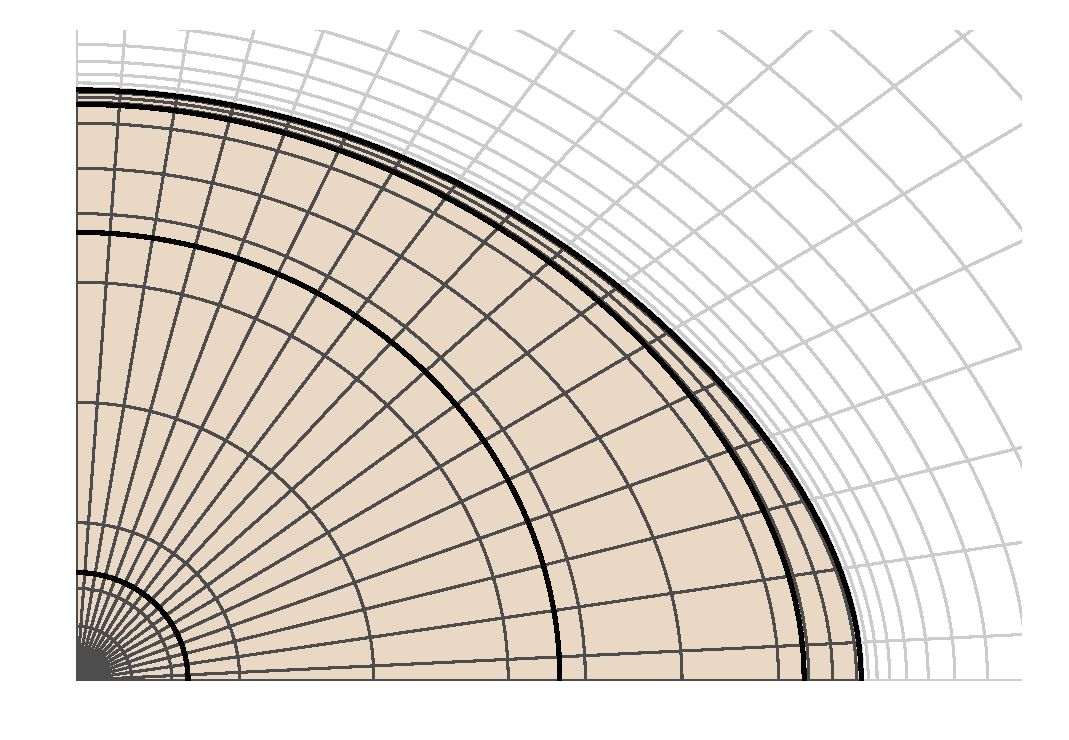
\includegraphics[width=0.8\textwidth]{fig/mapping.eps}
\caption{Coordinate mapping.}
\end{figure}


We use a technique adopted from \citet{Bonazzola}, in each subdomain
$\mathcal{D}_i$ we use a mapping in the form

\begin{equation}
\label{eq:map}
r(\zeta,\theta)=a_i\xi\Delta\eta_i+R_i(\theta)+A_i(\xi)(\Delta R_i(\theta)-a_i\Delta\eta_i) 
\qquad \mbox{for $\zeta\in[\eta_i,\eta_{i+1}]$}
\end{equation}
where we have defined:
\begin{eqnarray*}
\eta_i&=&R_i(\theta=0)\\
\Delta\eta_i&=&\eta_{i+1}-\eta_i\\
\Delta R_i(\theta)&=&R_{i+1}(\theta)-R_{i}(\theta)\\
\xi&=&\displaystyle\frac{\zeta-\eta_i}{\Delta\eta_i}
\end{eqnarray*} 

The function(s) $A_i(\xi)$ and the constant(s) $a_i$ determine the final
form of the mapping. In particular, the function $A_i(\xi)$ should verify
the following conditions:

\begin{eqnarray*}
r(\eta_i,\theta)=R(\theta) &\longrightarrow& A_i(\xi=0)=0\\
r(\eta_{i+1},\theta)=R_{i+1}(\theta) &\longrightarrow& A_i(\xi=1)=1
\end{eqnarray*}
The simplest possibility is a linear mapping

\begin{equation}
A_i(\xi)=\xi \qquad a_i=0
\end{equation}
that gives

\begin{equation}
\label{eq:map_linear}
r(\zeta,\theta)=R_i(\theta)+\xi\Delta R_i(\theta)
\end{equation}
But \citet{BGM98} proposed a mapping that satisfies some
extra conditions to make it suitable for spectral methods. For that
reason they set $A_i'(\xi=0)=0$ and $A_i'(\xi=1)=0$. Doing this, the
first derivative of the mapping

\begin{equation}
r_\zeta=\frac{\partial r}{\partial\zeta}=a_i+A_i'(\xi)\left(\frac{\Delta R_i(\theta)}{\Delta\eta_i}-a_i\right)
\end{equation}
is constant over the boundaries of the domains. This facilitates the
writing of interface conditions for the derivatives of the variables
in the problem when they are expressed in terms of their spectral
coefficients.  In this case, we will set

\begin{eqnarray}
\label{eq:map_bonazzola}
A_i(\xi)=-2\xi^3+3\xi^2 &\qquad& \mbox{for $i=1,\ldots,n-1$}\\
A_0(\xi)=-1.5\xi^5+2.5\xi^3&&
\end{eqnarray}
The constant $a_i$ deserves some special attention. We want $r_\zeta>0$,
that is, $r$ being monotonically increasing with $\zeta$, then $a_i$
should satisfy the condition

\begin{equation}
a_i(A_i'(\xi)-1)<A_i'(\xi)\frac{\Delta R_i(\theta)}{\Delta\eta_i}
\end{equation}
For $A_i'(\xi)=0$ (the boundaries), the condition states $a_i>0$.
When $A'(\xi)<1$, the condition is automatically satisfied (note that
$A_i'(\xi)$ is always positive).  But, since $A(\xi)$ should go from 0 at
$\xi=0$ to 1 at $\xi=1$, we know that $\max(A_i'(\xi))\ge1$, where the
equality corresponds to the linear mapping that we have seen before. So,
in the worst case, the condition becomes

\begin{equation}
a_i<\frac{1}{1-1/\max(A_i'(\xi))}\frac{\min(\Delta R_i(\theta))}{\Delta\eta_i}
\end{equation}
or, using (\ref{eq:map_bonazzola})

\begin{equation}
\begin{array}{l}
\displaystyle a_i<3\frac{\min(\Delta R_i(\theta))}{\Delta\eta_i} \qquad \mbox{for $i=1,\ldots,n-1$}\\
\displaystyle a_0<\frac{15}{7}\frac{\min(\Delta R_0(\theta))}{\Delta\eta_0}
\end{array}
\label{cdtstab}
\end{equation}
In practice, we take $a_i=1$. This is motivated by the fact that
we work with oblate domains. Indeed, the flattening increases for
the successive subdomains so that $\min(\Delta R_i(\theta))=\Delta
R_i(0)=\Delta\eta_i$. Hence, conditions \eq{cdtstab} are fully satisfied.

In addition, working with a fixed value of $a_i$ makes easier to work
with problems where the frontiers between the subdomains are not known
a priori, and the jacobian of the mapping becomes a smooth function
suitable for iterative methods.

The general form of the jacobian of the mapping is defined by the expression

\begin{equation}
\delta r^{i}=J_0^{(i)}(\zeta,\theta)\delta\eta_i+J_1^{(i)}(\zeta,\theta)\delta\Delta\eta_i
+J_2^{(i)}(\zeta,\theta)\delta R_i(\theta)+J_3^{(i)}(\zeta,\theta)\delta\Delta R_i(\theta)
\end{equation}
and using (\ref{eq:map}), for fixed $a_i$

\begin{equation}
\begin{array}{l}
J_0^{(i)}=0\\
J_1^{(i)}=a_i(\xi-A_i(\xi))\\
J_2^{(i)}=1\\
J_3^{(i)}=A_i(\xi)
\end{array}
\end{equation}

For the external domain, we will take 
\begin{equation}
\xi_{ex}=\frac{\zeta-\eta_n}{\eta_n} \qquad \xi\in[0,\infty)
\end{equation}
and

\begin{equation}
r_{ex}(\zeta,\theta)=\xi+R(\theta)
\end{equation}
with jacobian

\begin{equation}
\begin{array}{l}
J_0^{(ex)}=0\\
J_1^{(ex)}=0\\
J_2^{(ex)}=1\\
J_3^{(ex)}=0
\end{array}
\end{equation}

\subsection{Spheroidal coordinates}

In the previous section, we have defined a system of spheroidal
coordinates ($\zeta$,$\theta'$,$\varphi'$), where $\theta'=\theta$ and
$\varphi'=\varphi$ correspond to the usual spherical coordinates and
$\zeta$ is defined by a relation $r=r(\zeta,\theta)$. These spheroidal
coordinates are non-orthogonal, which means that the surfaces of constant
$\zeta$ are not perpendicular to those of constant $\theta$.

Before we continue, we should clarify a point. We have set
$\theta'=\theta$, so hereafter we will remove the tilde ($'$) to simplify
the notation. But when working with spheroidal coordinates, the partial
derivative $\frac{\partial}{\partial\theta}$ refers to the derivative
with respect to $\theta$ with $\zeta$ constant, that is not the habitual
derivative in spherical coordinates that is done holding $r$ constant.

$$\left.\frac{\partial}{\partial\theta}\right|_{\zeta,\varphi\,\mathrm{const.}}\ne
\left.\frac{\partial}{\partial\theta}\right|_{r,\varphi\,\mathrm{const.}}$$

The same can be said for the azimuthal coordinate $\varphi$ but, in this case
$\left.\frac{\partial}{\partial\varphi}\right|_{\zeta,\theta\,\mathrm{const.}}=
\left.\frac{\partial}{\partial\varphi}\right|_{r,\theta\,\mathrm{const.}}$.

\subsubsection{Natural basis}

We will start by defining the natural basis for the spheroidal coordinates, we have two sets of basis vectors:
\begin{itemize}
\item Covariant basis vectors: $\displaystyle\vect{E}_i=\frac{\partial\vect r}
{\partial x^i}$
\begin{equation}
\vect E_\zeta=r_\zeta\rvec, \quad
\vect E_\theta=r_\theta\rvec+r\thvec, \quad
\vect E_\varphi=r\sin\theta\phivec,
\end{equation}
\item Contravariant basis vectors: $\vect E^i=\nabla x^i$
\begin{equation}
\vect E^\zeta=\frac{\rvec}{r_\zeta}-\frac{r_\theta}{rr_\zeta}\thvec, \quad
\vect E^\theta=\frac{\thvec}{r},\quad
\vect E^{\varphi}=\frac{\phivec}{r\sin\theta},
\end{equation}
\end{itemize}
\noindent where $\rvec,\thvec,\phivec$ are the usual unit vectors in spherical coordinates, and
$$r_\zeta=\frac{\partial r}{\partial\zeta}\quad r_\theta=\frac{\partial r}{\partial\theta}$$

The vectors of the natural basis are not unit vectors. The covariant vector $\vect E_i$ is parallel to 
the line $x^j=\mathrm{const.}$ with $j\ne i$, while the contravariant vector $\vect E^i$ is 
perpendicular to the surface $x^i=\mathrm{const.}$ For orthogonal coordinates $\vect E_i\parallel\vect E^i$, but
this is not the case for non-orthogonal coordinates.

\begin{center}
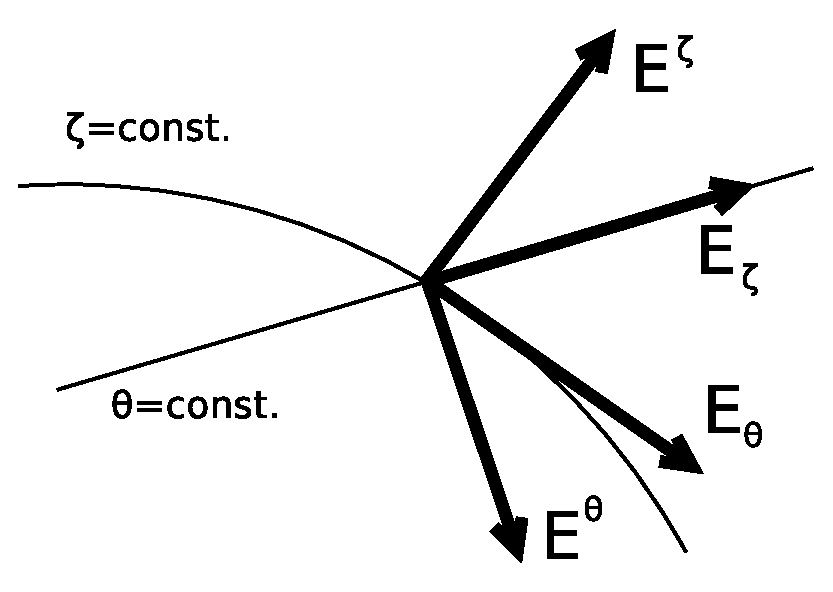
\includegraphics[width=5cm]{fig/vectors.eps}
\end{center}

The basis vectors satisfy
\begin{equation}
\vect E_i\cdot\vect E^j=\vect E^i\cdot\vect E_j=\delta_{ij}
\end{equation}
where $\delta_{ij}$ is the Kronecker's delta.

Using the basis vectors, we can calculate the metric tensor
\begin{equation}
g_{ij}=\vect E_i\cdot\vect E_j=\left(
\begin{array}{ccc}
r_\zeta^2&r_\zeta r_\theta&0\\
r_\zeta r_\theta&r^2+r_\theta^2&0\\
0&0&r^2\sin^2\theta
\end{array}
\right)
\end{equation}
or, in contravariant form
\begin{equation}
g^{ij}=\vect E^i\cdot\vect E^j=\left(
\begin{array}{ccc}
\displaystyle\frac{r^2+r_\theta^2}{r^2r_\zeta^2}&\displaystyle\frac{-r_\theta}{r^2r_\zeta}&0\\
\displaystyle\frac{-r_\theta}{r^2r_\zeta}&\displaystyle\frac{1}{r^2}&0\\
0&0&\displaystyle\frac{1}{r^2\sin^2\theta}
\end{array}
\right)
\end{equation}
Note that $g^{ij}$ is the matrix inverse of $g_{ij}$
$$g_{ij}g^{jk}=\delta_{ij}$$
where we have used the Einstein's summation convention, that implies summation over repeated indices.

Given two points $x^i$ and $x^i+\mathrm{d}x^i$, the distance ($\mathrm{d}s$) between them 
is given by the metric tensor:
\begin{equation}
\mathrm{d}s^2=g_{ij}\mathrm{d}x^i\mathrm{d}x^j=
r_\zeta^2\mathrm{d}\zeta^2+2r_\zeta r_\theta \mathrm{d}\zeta \mathrm{d}\theta+
(r^2+r_\theta^2)\mathrm{d}\theta^2+r^2\sin^2\theta \mathrm{d}\varphi^2
\end{equation}

The basis vectors verify
\begin{equation}
\vect E_i\cdot(\vect E_j\times\vect E_k)=\epsilon_{ijk}
\end{equation}
and
\begin{equation}
\vect E^i\cdot(\vect E^j\times\vect E^k)=\epsilon^{ijk}
\end{equation}
where $\epsilon^{ijk}$ is the Levi-Civita tensor
\begin{equation}
\epsilon_{ijk}=\sqrt{|g|}[i,j,k]
\end{equation}
\begin{equation}
\epsilon^{ijk}=\frac{1}{\sqrt{|g|}}[i,j,k]
\end{equation}
where $|g|=\det(g_{ij})=r^4r_\zeta^2\sin^2\theta$ and
\begin{equation}
[i,j,k]=\left\{
\begin{array}{ll}
1&\quad\mbox{the arguments are an even permutation}\\
-1&\quad\mbox{the arguments are an odd permutation}\\
0&\quad\mbox{two or more arguments are equal}
\end{array}
\right.
\end{equation}


\subsubsection{Representation of vectors}

A vector $\vect v$ can be represented either in covariant or contravariant form:
\begin{itemize}
\item Covariant form: $\vect v=V_\zeta\vect E^\zeta+V_\theta\vect E^\theta+V_\varphi\vect E^\varphi$
\item Contravariant form: $\vect v=V^\zeta\vect E_\zeta+V^\theta\vect E_\theta+V^\varphi\vect E_\varphi$
\end{itemize}
Here, $V_i$ are the covariant components of the vector $\vec v$ and $V^i$ the contravariant components. Note that
$$\vect E_i\cdot\vect v=V_i \qquad \mbox{and} \qquad \vect E^i\cdot\vect v=V^i$$
We can use the metric tensor to pass from one representation to the other, indeed
\begin{equation}
V_i=\vect E_i\cdot\vect v=\vect E_i\cdot(\vect E_j V^j)=g_{ij}V^j
\end{equation}
and similarly
\begin{equation}
V^i=g^{ij}V_j
\end{equation}

Let $(v_r,v_\theta,v_\varphi)$ be the spherical components of a vector $\vect v$ such that
$\vect v=v_r\rvec+v_\theta\thvec+v_\varphi\phivec$. Its spheroidal components will be
\begin{equation}
V_\zeta=r_\zeta v_r,\quad V_\theta=r_\theta v_r+r v_\theta,\quad
V_\varphi=r\sin\theta v_\varphi
\end{equation}
and
\begin{equation}
V^\zeta=\frac{v_r}{r_\zeta}-\frac{r_\theta}{rr_\zeta}v_\theta,\quad
V^\theta=\frac{v_\theta}{r},\quad V^\varphi=\frac{v_\varphi}{r\sin\theta}
\end{equation}
We can see from this expressions that $V^\theta$ an $V^\varphi$ are in fact angular velocities.


Using the properties of the basis vectors it can be shown that the scalar product of two vectors is
given by
\begin{equation}
\vect a\cdot\vect b=A_iB^i=A^iB_i
\end{equation}
and the cross product is
\begin{equation}
\begin{array}{l}
(\vect a\times\vect b)^i=
\epsilon^{ijk}A_jB_k\\
(\vect a\times\vect b)_i=
\epsilon_{ijk}A^jB^k
\end{array}
\end{equation}

We have presented the basics of the representation of vectors in spheroidal coordinates, let'see now a little
example. Consider a surface $\mathcal S$ defined by $\zeta=\mathrm{const.}$ as for example the surface
of a star or the frontier between two subdomains. We want to calculate the normal and tangential
projections of a vector $\vect v$ with respect to $\mathcal{S}$. First, we define a unit vector $\vect{\hat n}$,
perpendicular to $\mathcal{S}$. For that, we just recall that $\vect E^\zeta$ is perpendicular to 
the surfaces $\zeta=\mathrm{const.}$, but it is not a unit vector, so
\begin{equation}
\vect{\hat n}=\frac{\vect{E^\zeta}}{|\vect{E^\zeta}|}=
\frac{\vect{E^\zeta}}{\sqrt{\vect{E^\zeta}\cdot\vect{E^\zeta}}}=
\frac{\vect{E^\zeta}}{\sqrt{g^{\zeta\zeta}}}
\end{equation}
then, the normal projection is
\begin{equation}
\vect{\hat n}\cdot\vect{v}=\frac{V^\zeta}{\sqrt{g^{\zeta\zeta}}}=
\frac{r_\zeta V^\zeta}{\sqrt{1+\frac{r_\theta^2}{r^2}}}
\end{equation}
For the parallel projection we have two vectors, the first one, in the direction of $\varphi$ is just 
the spherical unit vector $\phivec$, in the latitudinal direction, however, it will be
\begin{equation}
\vect{\hat t}=\frac{\vect{E_\theta}}{|\vect{E_\theta}|}=
\frac{\vect{E_\theta}}{\sqrt{\vect{E_\theta}\cdot\vect{E_\theta}}}=
\frac{\vect{E_\theta}}{\sqrt{g_{\theta\theta}}}
\end{equation}
so, the parallel projections over $\mathcal{S}$ are
\begin{equation}
\vect{\hat t}\cdot\vect{v}=\frac{V_\theta}{\sqrt{g_{\theta\theta}}}=
\frac{1}{\sqrt{1+\frac{r_\theta^2}{r^2}}}\frac{V_\theta}{r}
\end{equation}
and
\begin{equation}
\phivec\cdot\vect{v}=\frac{V_\varphi}{r\sin\theta}
\end{equation}

\subsubsection{Tensors}

A second order tensor $\tens T$ is represented using 2 indices
\begin{equation}
\tens T=T^{ij}\vect E_i\vect E_j=T_{ij}\vect E^i\vect E^j={T^i}j\vect E_i\vect E^j
={T_i}^j\vect E^i\vect E_j
\end{equation}
Again, we can use the metric tensor to lower and raise indices
\begin{equation}
\begin{array}{l}
T^{ij}=g^{ik}{T_k}^j=g^{jl}{T^i}_l=g^{ik}g^{jl}T_{kl}\\
T_{ij}=g_{ik}{T^k}_j=g_{jl}{T_i}^l=g_{ik}g_{jl}T^{kl}
\end{array}
\end{equation}

The tensor product of 2 vectors is a tensor
\begin{equation}
(\vect a\;\vect b)^{ij}=a^ib^j
\end{equation}
The dot product between a tensor and a vector is
\begin{equation}
(\tens T\cdot\vect v)^i=T^{ij}V_j
\end{equation}
and between a vector and a tensor
\begin{equation}
(\vect v\cdot\tens T)^j=T^{ij}V_i
\end{equation}
Finally, the double dot product is a scalar
\begin{equation}
\tens T : \tens T=T^{ij}T_{ij}
\end{equation}

All of this can be generalized to higher order tensors. Note that vectors are in fact tensors of order 1. 

\subsubsection{Differential operators}

Our goal is to be able to write differential equations using spheroidal coordinates. We will start
finding the relation between the partial derivatives with respect to the spherical coordinates and those
calculated with respect to the spheroidal coordinates. We will add the primes ($'$) in the notation for 
the spheroidal $\theta'$ and $\varphi'$ coordinates to clarify the notation, so the derivative with
respect to a spheroidal coordinate is done holding the other spheroidal coordinates constant.
Following the chain rule
\begin{equation}
\frac{\partial}{\partial r}=
\frac{\partial\zeta}{\partial r}\frac{\partial}{\partial \zeta}
+\frac{\partial\theta'}{\partial r}\frac{\partial}{\partial \theta'}
+\frac{\partial\varphi'}{\partial r}\frac{\partial}{\partial \varphi'}
\end{equation}
Obviously, $\displaystyle \frac{\partial\theta'}{\partial r}=\frac{\partial\varphi'}{\partial r}=0$, and
$$\mathrm{d}r=r_\zeta\mathrm{d}\zeta+r_\theta\mathrm{d}\theta$$
$$\mathrm{d}\zeta=\frac{1}{r_\zeta}\mathrm{d}r-\frac{r_\theta}{r_\zeta}\mathrm{d}\theta$$
where we see $\displaystyle \frac{\partial\zeta}{\partial r}=\frac{1}{r_\zeta}$
and $\displaystyle \frac{\partial\zeta}{\partial\theta}=-\frac{r_\theta}{r_\zeta}$. Then
\begin{equation}
\frac{\partial}{\partial r}=\frac{1}{r_\zeta}\frac{\partial}{\partial \zeta}
\end{equation}
The other partial derivatives are calculated in the same way
\begin{equation}
\frac{\partial}{\partial\theta}=\frac{\partial}{\partial \theta'}
-\frac{r_\theta}{r_\zeta}\frac{\partial}{\partial \zeta}
\end{equation}
\begin{equation}
\frac{\partial}{\partial \varphi}=\frac{\partial}{\partial \varphi'}
\end{equation}
Of course, we could take this expressions and substitute them into the expressions for the differential
operators corresponding to the spherical coordinates, but there is a much more efficient way to do it.

First, let's define the general form of the gradient of a scalar quantity. The gradient will be a vector,
whose covariant components are
\begin{equation}
(\nabla\phi)_i=\frac{\partial\phi}{\partial x^i}=\phi_{,i}
\end{equation}
where we have introduced the comma notation for the partial derivative. The contravariant components of 
the gradient will be
\begin{equation}
(\nabla\phi)^i=g^{ij}\phi_{,j}
\end{equation}

We can also derive a component of a vector $V^i$ in the same way. However, this derivative
\begin{equation}
\frac{\partial V^i}{\partial x^j}={V^i}_{,j}
\end{equation}
is not a tensor, as it does not transform correctly under a change of coordinates. That's why we will introduce
the covariant derivative
\begin{equation}
\nabla_jV^i={V^i}_{;j}={V^i}_{,j}+{\Gamma^i}_{kj}V^k
\end{equation}
Where $\displaystyle{\Gamma^i}_{kj}=\vect E^i\cdot\frac{\partial \vect E_k}{\partial x^j}$
is a Christoffel symbol of the second kind. The covariant derivative of a vector ${V^i}_{;j}$ is a tensor
that represents the gradient of the vector.
\begin{equation}
(\nabla\vect v)^{ij}=g^{jk}{(\nabla\vect v)^i}_k=g^{jk}{V^i}_{;k}
\end{equation}
We can also calculate the covariant derivative using the covariant components of the vector
\begin{equation}
\nabla_jV_i={V_i}_{;j}={V_i}_{,j}-{\Gamma^k}_{ij}V_k
\end{equation}

The Christoffel symbols can be calculated using the following relation
\begin{equation}
\Gamma^i_{jk}=
\frac{1}{2}g^{il}(g_{lj,k}+g_{lk,j}-g_{jk,l})
\end{equation}
where we can see that they are symmetric with respect to the second and third indices $\Gamma^i_{jk}=\Gamma^i_{kj}$.
They also verify
\begin{equation}
\Gamma^{i}_{ji}=\frac{\log\sqrt{|g|}}{\partial x^j}
\end{equation}

The covariant derivative of second order tensors is done in a similar way
\begin{equation}
\nabla_kT^{ij}={T^{ij}}_{;k}={T^{ij}}_{,k}+{\Gamma^i}_{lk}T^{lj}+{\Gamma^j}_{lk}T^{il}
\end{equation}
If one of the indices is covariant, then we do
\begin{equation}
\nabla_k{T^i}_j={{T^i}_j}_{;k}={{T^i}_j}_{,k}+{\Gamma^i}_{lk}{T^l}_j-{\Gamma^l}_{jk}{T^i}_l
\end{equation}
where we can see the general rule valid also for higher order tensors, the covariant derivative is equal
to the regular derivative plus:
\begin{itemize}
\item For each contravariant index, we add ${\Gamma^i}_{lk}T^{\ldots l\ldots}$
\item For each covariant index, we subtract ${\Gamma^l}_{ik}T_{\ldots l\ldots}$
\end{itemize}

Using the covariant derivative, we can calculate all the differential operators in spheroidal coordinates.
We have already see the gradient of a scalar and a vector, similarly, the divergence of a vector will be
\begin{equation}
\nabla\cdot\vect v=\nabla_iV^i={V^i}_{;i}
\end{equation}
and for a tensor
\begin{equation}
(\nabla\cdot\tens T)^i=\nabla_jT^{ij}={T^{ij}}_{;j}
\end{equation}
Note that some authors prefer the definition $(\nabla\cdot\tens T)^j=\nabla_iT^{ij}={T^{ij}}_{;i}$.
Using the expresion for the cross product, we can calculate the curl of a vector
\begin{equation}
(\nabla\times\vect v)^i=\epsilon^{ijk}\nabla_jV_k=\epsilon^{ijk}{V_k}_{;j}
\end{equation}
The laplacian of a scalar field will be
\begin{equation}
\Delta\phi=\nabla\cdot(\nabla\phi)=\nabla_i(g^{ij}\nabla_j\phi)=(g^{ij}\phi_{,j})_{;i}
\end{equation}
and for a vector field
\begin{equation}
(\Delta\vect v)^i=\nabla_j(g^{jk}\nabla_kV^i)=(g^{jk}{V^i}_{;k})_{;j}
\end{equation}
The material derivative is
\begin{equation}
\left[(\vect v\cdot\nabla)\vect v\right]^i=V^j\nabla_jV^i=V^j{V^i}_{;j}
\end{equation}

\subsubsection{Useful relations}
\begin{itemize}
\item Line, area and volume elements
\begin{itemize}
\item Line element
\begin{equation}
\mathrm{d}s^2=g_{ij}\mathrm{d}x^i\mathrm{d}x^j=r_\zeta^2\mathrm{d}\zeta^2+2r_\zeta r_\theta \mathrm{d}\zeta \mathrm{d}\theta+
(r^2+r_\theta^2)\mathrm{d}\theta^2+r^2\sin^2\theta \mathrm{d}\varphi^2
\end{equation}
\begin{equation}
\mathrm{d}\vect r=\vect E_i \mathrm{d}x^i=\vect E_\zeta \mathrm{d}\zeta+\vect E_\theta \mathrm{d}\theta
+\vect E_\varphi \mathrm{d}\varphi
\end{equation}
\item Area element in a surface $\zeta=$const.
\begin{equation}
\mathrm{d}\vect S=(\vect E_\theta\times \vect E_\varphi)\mathrm{d}\theta \mathrm{d}\varphi=
r^2r_\zeta\sin\theta\vect E^\zeta \mathrm{d}\theta \mathrm{d}\varphi
\end{equation}
\begin{equation}
\mathrm{d}S=|\mathrm{d}\vect S|=
\sqrt{g^{\zeta\zeta}}r^2r_\zeta\sin\theta \mathrm{d}\theta \mathrm{d}\varphi=
r^2\sqrt{1+\frac{r_\theta^2}{r^2}}\sin\theta \mathrm{d}\theta \mathrm{d}\varphi
\end{equation}
\item Area element in a surface of constant $p=p(\zeta,\theta)$.
\begin{equation}
\mathrm{d}\vect S=
r^2r_\zeta\sin\theta\left(\vect E^\zeta+\frac{p_{,\theta}}{p_{,\zeta}}\vect E^{\theta}
\right) \mathrm{d}\theta \mathrm{d}\varphi
\end{equation}
\begin{equation}
\mathrm{d}S=|\mathrm{d}\vect S|=r^2r_\zeta\sin\theta
\sqrt{g^{\zeta\zeta}+2\frac{p_{,\theta}}{p_{,\zeta}}g^{\zeta\theta}
+\left(\frac{p_{,\theta}}{p_{,\zeta}}\right)^2g^{\theta\theta}}
\mathrm{d}\theta \mathrm{d}\varphi
\end{equation}
\item Volume element
\begin{equation}
\mathrm{d}V=\vect E_\zeta\cdot(\vect E_\theta\times\vect E_\varphi)\mathrm{d}\zeta \mathrm{d}\theta \mathrm{d}\varphi=
r^2r_\zeta\sin\theta \mathrm{d}\zeta \mathrm{d}\theta \mathrm{d}\varphi
\end{equation}
\end{itemize}
\item Differential operators
\begin{itemize}
\item Gradient
\begin{equation}
\nabla\phi=\phi_{,i}\vect E^i=\frac{\partial\phi}{\partial\zeta}\vect E^\zeta+
\frac{\partial\phi}{\partial\theta}\vect E^\theta+\frac{\partial\phi}{\partial\varphi}\vect E^\varphi
\end{equation}
\item Divergence
\begin{equation}
\begin{array}{rl}
\displaystyle\nabla\cdot\vect v&
\displaystyle ={V^i}_{;i}=
\frac{\partial V^i}{\partial x^i}+\frac{\partial\log\sqrt{|g|}}{\partial x^k}V^k=\\
\\
&\displaystyle =\frac{\partial V^\zeta}{\partial\zeta}+\left(\frac{2r_\zeta}{r}
+\frac{r_{\zeta\zeta}}{r_\zeta}
\right)V^\zeta+\frac{\partial V^\theta}{\partial\theta}+\left(\frac{2r_\theta}{r}+
\frac{\cos\theta}{\sin\theta}+\frac{r_{\zeta\theta}}{r_\zeta}\right)V^\theta+
\frac{\partial V^\varphi}{\partial\varphi}
\end{array}
\end{equation}
\item Laplacian
\begin{equation}
\begin{array}{rl}
\Delta\phi&
\displaystyle =\div(\nabla\phi)=(g^{ij}\phi_{,j})_{;i}=\frac{1}{\sqrt{|g|}}\frac{\partial}{\partial x^i}
\left(\sqrt{|g|}g^{ij}\frac{\partial\phi}{\partial x^j}\right)=\\
\\
&\displaystyle =
g^{\zeta\zeta}\frac{\partial^2\phi}{\partial\zeta^2}
+2g^{\zeta\theta}\frac{\partial^2\phi}{\partial\zeta\partial\theta}
+\frac{1}{r^2}\frac{\partial^2\phi}{\partial\theta^2}
+\frac{1}{r^2\sin^2\theta}\frac{\partial^2\phi}{\partial\varphi^2}
+\\
&\displaystyle\quad
+\left[\frac{2}{rr_\zeta}-\frac{r_{\theta\theta}}{r^2r_\zeta}
-g^{\zeta\zeta}\frac{r_{\zeta\zeta}}{r_\zeta}
-g^{\zeta\theta}\left(\frac{2r_{\zeta\theta}}{r_\zeta}-\frac{\cos\theta}{\sin\theta}\right)\right]
\frac{\partial\phi}{\partial\zeta}
+\frac{\cos\theta}{r^2\sin\theta}\frac{\partial\phi}{\partial\theta}
\end{array}
\end{equation}
\item Curl
\begin{equation}
\begin{array}{rl}
\displaystyle \nabla\times\vect v &
\displaystyle = \epsilon^{ijk}V_{k;j}\vect E_i=\\
\\
&\displaystyle = \frac{1}{r^2r_\zeta\sin\theta}\left[
\left(\frac{\partial V_\varphi}{\partial\theta}-
\frac{\partial V_\theta}{\partial\varphi}\right)\vect E_\zeta +
\left(\frac{\partial V_\zeta}{\partial\varphi}-
\frac{\partial V_\varphi}{\partial\zeta}\right)\vect E_\theta +
\left(\frac{\partial V_\theta}{\partial\zeta}-
\frac{\partial V_\zeta}{\partial\theta}\right)\vect E_\varphi\right]\\
\end{array}
\end{equation}
\item Material derivative
\begin{equation}
\begin{array}{l}
\displaystyle(\vect a\cdot\nabla)\vect b
 =A^j{B^i}_{;j}\vect E_i=\\
\\
\quad\displaystyle =\left[A^\zeta\frac{\partial B^\zeta}{\partial\zeta}+
A^\theta\frac{\partial B^\zeta}{\partial\theta}+A^\varphi\frac{\partial B^\zeta}{\partial\varphi}
+\frac{r_{\zeta\zeta}}{r_\zeta}A^\zeta B^\zeta+\left(\frac{r_{\zeta\theta}}{r_\zeta}-\frac{r_\theta}{r}
\right)\left(A^\zeta B^\theta+A^\theta B^\zeta\right)+\right.\\
\quad\displaystyle \left. +\frac{1}{r_\zeta}\left(r_{\theta\theta}-
\frac{2r_\theta^2}{r}-r\right)A^\theta B^\theta+\frac{\sin\theta}{r_\zeta}\left(
r_\theta\cos\theta-r\sin\theta\right)A^\varphi B^{\varphi}\right]\vect E_\zeta +\\
\\
\quad\displaystyle +\left[A^\zeta\frac{\partial B^\theta}{\partial\zeta}+
A^\theta\frac{\partial B^\theta}{\partial\theta}+A^\varphi\frac{\partial B^\theta}{\partial\varphi}
+\frac{r_\zeta}{r}\left(A^\zeta B^\theta+A^\theta B^\zeta\right)
+\frac{2r_\theta}{r}A^\theta B^\theta-
\sin\theta\cos\theta A^\varphi B^{\varphi}\right]\vect E_\theta +\\
\\
\quad\displaystyle +\left[A^\zeta\frac{\partial B^\varphi}{\partial\zeta}+
A^\theta\frac{\partial B^\varphi}{\partial\theta}+A^\varphi\frac{\partial B^\varphi}{\partial\varphi}
+\frac{r_\zeta}{r}\left(A^\zeta B^\varphi+A^\varphi B^\zeta\right)
+\left(\frac{r_\theta}{r}+\frac{\cos\theta}{\sin\theta}\right)
\left(A^\theta B^\varphi+A^\varphi B^\theta\right)\right]\vect E_\varphi\\
\end{array}
\end{equation}
\end{itemize}
\item Christoffel symbols (different from 0)
\begin{equation}
\begin{array}{lll}
\displaystyle
\Gamma^{\zeta}_{\zeta\zeta}=\frac{r_{\zeta\zeta}}{r_\zeta}&
\displaystyle
\Gamma^{\zeta}_{\zeta\theta}=\Gamma^{\zeta}_{\theta\zeta}=
\frac{r_{\zeta\theta}}{r_\zeta}-\frac{r_\theta}{r}&
\displaystyle
\Gamma^{\zeta}_{\theta\theta}=\frac{1}{r_\zeta}\left(r_{\theta\theta}-
\frac{2r_\theta^2}{r}-r\right)\\
\displaystyle
\Gamma^{\zeta}_{\varphi\varphi}=\frac{\sin\theta}{r_\zeta}(r_\theta\cos\theta
-r\sin\theta)&
\displaystyle
\Gamma^{\theta}_{\zeta\theta}=\Gamma^{\theta}_{\theta\zeta}=\frac{r_\zeta}{r}&
\displaystyle
\Gamma^{\theta}_{\theta\theta}=\frac{2r_{\theta}}{r}\\
\displaystyle
\Gamma^{\theta}_{\varphi\varphi}=-\sin\theta\cos\theta&
\displaystyle
\Gamma^{\varphi}_{\zeta\varphi}=\Gamma^{\varphi}_{\varphi\zeta}=\frac{r_\zeta}{r}&
\displaystyle
\Gamma^{\varphi}_{\theta\varphi}=\Gamma^{\varphi}_{\varphi\theta}=\frac{r_\theta}{r}+
\frac{\cos\theta}{\sin\theta}
\end{array}
\end{equation}

\end{itemize}

\subsection{Multidomain and continuity conditions}

When using multidomain we will deal with the problem of writing continuity conditions for the different variables
on the boundaries between contiguous subdomains. The main issue is that the mapping presented in \ref{sect:mapping}
have discontinuities in some of its derivatives, so we should take care of using the correct expressions for
this conditions. 

\begin{center}
\begin{tabular}{c|c|c}
& \multicolumn{2}{c}{Continuous between subdomains} \\
& Bonazzola & Linear mapping \\
\hline
$r$ & Yes & Yes\\
$r_\zeta$ & No (Yes for fixed $a_i$) & No\\
$r_{\zeta\zeta}$ & No & Yes \\
$r_\theta$ & Yes & Yes \\
$r_{\theta\theta}$ & Yes & Yes \\
$r_{\zeta\theta}$ & Yes & No \\
\end{tabular}
\end{center}

In the case of a scalar field $\phi(r,\theta)$, if $\phi$ is continuous between subdomains, the condition is easy
\begin{equation}
\phi^{(+)}=\phi^{(-)}
\end{equation}
where $(+)$ and $(-)$ represent each side of the boundary. If we want $\phi$ to be derivable across the boundary, 
we would write a condition for the normal derivative $\vect{\hat n}\cdot\nabla\phi$ and not for 
$\frac{\partial\phi}{\partial\zeta}$,
\begin{equation}
\label{eq:map_cond_der}
\vect{\hat n}\cdot\nabla^{(+)}\phi^{(+)}=\vect{\hat n}\cdot\nabla^{(+)}\phi^{(+)}
\end{equation}
where 
\begin{equation}
\begin{array}{rl}
\vect{\hat n}\cdot\nabla\phi&
\displaystyle =\frac{\vect E^\zeta}{\sqrt{g^{\zeta\zeta}}}\cdot\left(\frac{\partial\phi}{\partial\zeta}\vect E^\zeta+
\frac{\partial\phi}{\partial\theta}\vect E^\theta+\frac{\partial\phi}{\partial\varphi}\vect E^\varphi\right)\\
&\\&
\displaystyle =\sqrt{g^{\zeta\zeta}}\frac{\partial\phi}{\partial\zeta}+\frac{g^{\zeta\theta}}{\sqrt{g^{\zeta\zeta}}}
\frac{\partial\phi}{\partial\theta}\\
&\\&
\displaystyle =\sqrt{1+\frac{r_\theta^2}{r^2}}\left(\frac{1}{r_\zeta}\frac{\partial\phi}{\partial\zeta}-
\frac{r_\theta}{r^2+r_\theta^2}\frac{\partial\phi}{\partial\theta}\right)
\end{array}
\end{equation}
We know that $r$ and $r_\theta$ are continuous across the boundary and if $\phi$ is continuous then so is
$\frac{\partial\phi}{\partial\theta}$, then the condition (\ref{eq:map_cond_der}) becomes
\begin{equation}
\frac{1}{r_\zeta^{(+)}}\left(\frac{\partial\phi}{\partial\zeta}\right)^{(+)}=
\frac{1}{r_\zeta^{(-)}}\left(\frac{\partial\phi}{\partial\zeta}\right)^{(-)}
\end{equation}
that is equivalent to saying $\displaystyle\left(\frac{\partial\phi}{\partial r}\right)^{(+)}=
\left(\frac{\partial\phi}{\partial r}\right)^{(-)}$.

In the case of a vector field, the conditions are
\begin{equation}
\begin{array}{c}
\displaystyle r_\zeta^{(+)} {V^\zeta}^{(+)}=r_\zeta^{(-)} {V^\zeta}^{(-)} \\
\displaystyle {V^\theta}^{(+)}={V^\theta}^{(-)} \\
\displaystyle {V^\varphi}^{(+)}={V^\varphi}^{(-)} 
\end{array}
\end{equation}
for continuity and
\begin{equation}
\begin{array}{c}
\displaystyle \left(\frac{\partial V^{\zeta}}{\partial\zeta}\right)^{(+)}
+\frac{1}{r_\zeta^{(+)}}\left(r_{\zeta\zeta}^{(+)}{V^\zeta}^{(+)}+r_{\zeta\theta}^{(+)}{V^\theta}^{(+)}\right)=
\left(\frac{\partial V^{\zeta}}{\partial\zeta}\right)^{(-)}
+\frac{1}{r_\zeta^{(-)}}\left(r_{\zeta\zeta}^{(-)}{V^\zeta}^{(-)}+r_{\zeta\theta}^{(-)}{V^\theta}^{(-)}\right) \\
\displaystyle \frac{1}{r_\zeta^{(+)}}\left(\frac{\partial V^{\theta}}{\partial\zeta}\right)^{(+)}= 
\frac{1}{r_\zeta^{(-)}}\left(\frac{\partial V^{\theta}}{\partial\zeta}\right)^{(-)} \\
\displaystyle \frac{1}{r_\zeta^{(+)}}\left(\frac{\partial V^{\varphi}}{\partial\zeta}\right)^{(+)}= 
\frac{1}{r_\zeta^{(-)}}\left(\frac{\partial V^{\varphi}}{\partial\zeta}\right)^{(-)}
\end{array}
\end{equation}
for derivability. These conditions are based on the fact that the spherical components of the vector field
are continuous and derivable scalar functions. For a physical boundary, it could happen that 
some components of the vector
field are continuous (or derivable) and others are not, then none of the above conditions is correct.

\pagebreak

\section{Coordinate mapping in ESTER}

The class \verb|mapping| combines a \verb|diff_gl| object with a \verb|diff_leg| object to perform 
calculations in 2D. The prototype of this class is defined in \verb|mapping.h|.

Let's see an example of initialization of a mapping object

\begin{minted}[frame=single]{cpp}
mapping map;

map.set_ndomains(3);
map.set_npts(20);
map.set_nt(25);
map.set_nex(20);
map.init();

map.R.setrow(1,0.5*ones(1,map.nt));
map.R.setrow(2,1+0.1*sin(map.th)*sin(map.th));
map.R.setrow(3,2+0.3*sin(map.th)*sin(map.th));

map.remap();

\end{minted} 
First, we have declared the object
\mint{cpp}|mapping map;|
Then we set the number of domains
\mint{cpp}|map.set_ndomains(3);|
Our mapping will have 3 domains plus one external domain. We choose the number of points in the internal
domains
\mint{cpp}|map.set_npts(20);|
That is, the 3 domains will have each one 20 points. We can also set a different number of points for
each domain, for that we should do
\begin{minted}{cpp}
int npts[3];
npts[0]=10;npts[1]=20;npts[2]=30;
map.set_npts(npts);
\end{minted}
After that, we set the number of points in latitude (25) and in the external domain (20)
\begin{minted}{cpp}
map.set_nt(25);
map.set_nex(20);
\end{minted}
If we are not using the external domain, there is no need to change its number of points (It is 10 by default).
There is one optional parameter that we can set before initialize the mapping
\mint{cpp}|map.mode=MAP_BONAZZOLA;|
to use the mapping with constant $r_\zeta$ at the boundaries presented in the previous section (this is
the default), or
\mint{cpp}|map.mode=MAP_LINEAR;|
to use a linear mapping. Now we can proceed with the initialization
\mint{cpp}|map.init();|
If we change the resolution after this point, we should call \verb|init()| again. Now
we have a working object, with 3 spherical domains distributed uniformly from $r=0$ to $r=1$.
If this setup is fine for us,
then we are done with the initialization, but usually we will want to change to boundaries between
domains. This is done using the matrix \verb|R| with size $(n_\mathrm{domains}+1)\times n_\theta$.
Each row of \verb|R| defines a different boundary, starting with the row 0 that corresponds to the inner boundary.
In the previous example, we have not changed the inner boundary, so our mapping contains the center of 
coordinates, but if we want the mapping to start, for example, at $r=0.3$, we could just add
\mint{cpp}|map.R.setrow(0,0.3*ones(1,map.nt));|
In the definition of the boundaries we have used \verb|map.th| that contains the values of the $\theta$ coordinate.
Once we have set the boundaries we just call \verb|remap()|
\mint{cpp}|map.remap();|
We can call \verb|remap()| as many times as we want if we need to change the boundaries again.

After the initialization, a \verb|mapping| object contains the following variables

\medskip

\renewcommand{\arraystretch}{1.3} 

\noindent\begin{longtable}{p{3.7cm}ccp{5cm}}
Name&Type&Size&Description\\
\hline
\texttt{ndomains}&\texttt{int}&&Number of domains\\
\texttt{nr}&\texttt{int}&&Number of radial points\\
\texttt{nt}&\texttt{int}&&Number of latitudinal points\\
\texttt{nex}&\texttt{int}&&Number of radial points in the external domain\\
\texttt{npts}&\texttt{int[ndomains]}&&Number of points in each domain\\
\texttt{R}&\texttt{matrix}&(ndomains+1,nt)&Domain boundaries\\
\texttt{eta}&\texttt{matrix}&(ndomains+1,nt)&R($\theta=0$)\\
\texttt{z}&\texttt{matrix}&(nr,1)& Spheroidal radial coordinate $\zeta$\\
\texttt{th}&\texttt{matrix}&(1,nt)& Colatitude $\theta$\\
\texttt{r}&\texttt{matrix}&(nr,nt)& Spherical radial coordinate $r$\\
\texttt{ex.r}&\texttt{matrix}&(nex,nt)& Spherical radial coordinate $r$ in
the external domain\\
\texttt{rz}, \texttt{rt}, \texttt{rzz}, \texttt{rtt}, \texttt{rzt}
&\texttt{matrix}&(nr,nt)
& $r_\zeta$, $r_\theta$, $r_{\zeta\zeta}$, $r_{\theta\theta}$, $r_{\zeta\theta}$\\
\texttt{ex.rz}, \texttt{ex.rt}, \texttt{ex.rzz}, \texttt{ex.rtt}, \texttt{ex.rzt}
&\texttt{matrix}&(nex,nt)
& $r_\zeta$, $r_\theta$, $r_{\zeta\zeta}$, $r_{\theta\theta}$, $r_{\zeta\theta}$
in the external domain\\
\texttt{gzz}, \texttt{gzt}, \texttt{gtt}&\texttt{matrix}&(nr,nt)&
Elements of the metric tensor $g^{\zeta\zeta}$, $g^{\zeta\theta}$ and $g^{\theta\theta}$ \\
\texttt{ex.gzz}, \texttt{ex.gzt}, \texttt{ex.gtt}&\texttt{matrix}&(nex,nt)&
Elements of the metric tensor $g^{\zeta\zeta}$, $g^{\zeta\theta}$ and $g^{\theta\theta}$ 
in the external domain\\
\texttt{D}&\texttt{matrix\_block\_diag}&(nr,nr)& Differentiation matrix $\frac{\partial}{\partial\zeta}$\\
\texttt{ex.D}&\texttt{matrix}&(nex,nex)& Differentiation matrix $\frac{\partial}{\partial\zeta}$ in
the external domain\\
\texttt{Dt}, \texttt{Dt\_11}, \texttt{Dt\_01}, \texttt{Dt\_10}&\texttt{matrix}&(nt,nt)&
Differentiation matrix $\frac{\partial}{\partial\theta}$ for each type of symmetry\\
\texttt{Dt2}, \texttt{Dt2\_11}, \texttt{Dt2\_01}, \texttt{Dt2\_10}&\texttt{matrix}&(nt,nt)&
Second order differentiation matrix $\frac{\partial^2}{\partial\theta^2}$ for each type of symmetry\\
\texttt{I}&\texttt{matrix}&(1,nr)&Integration matrix $\int_{\eta_0}^{\eta_\mathrm{ndom.}}\mathrm{d}\zeta$\\
\texttt{It}&\texttt{matrix}&(nt,1)&Integration matrix $\int_0^\pi\sin\theta\mathrm{d}\theta$ for symmetric functions\\
\texttt{J}&\texttt{matrix[4]}&(nr,nt)&Jacobian of the mapping\\
\texttt{ex.J}&\texttt{matrix[4]}&(nex,nt)&Jacobian of the mapping in the external
domain\\
\texttt{gl}&\texttt{diff\_gl}&&Numerical differentiation object for the radial direction\\
\texttt{ex.gl}&\texttt{diff\_gl}&&Numerical differentiation object for the radial direction in the
external domain\\
\texttt{leg}&\texttt{diff\_leg}&&Numerical differentiation object for the latitudinal direction\\
\end{longtable}

\renewcommand{\arraystretch}{1} 

A given scalar field $\phi(\zeta,\theta)$ will be represented by a 2D matrix with size \verb|nr|$\times$\verb|nt|,
each element being the value of the function at each collocation point $\phi_{ij}=\phi(\zeta_i,\theta_j)$.
With this representation, the operators acting on the radial direction are implemented using left multiplication
while those acting in the latitudinal direction use right multiplication. Let's see some examples

\medskip
\renewcommand{\arraystretch}{2} 
\begin{tabular}{c@{\quad:\quad}c}
$\displaystyle\frac{\partial\phi}{\partial\zeta}$&\verb|(map.D,phi)|\\
$\displaystyle\int_{\eta_0}^{\eta_\mathrm{ndom.}}\phi\,\mathrm{d}\zeta$&\verb|(map.I,phi)|\\
$\displaystyle\frac{\partial\phi}{\partial\theta}$&\verb|(phi,map.Dt)|\\
$\displaystyle\int_0^\pi\phi\sin\theta\,\mathrm{d}\theta$&\verb|(phi,map.It)|\\
\end{tabular} 
\renewcommand{\arraystretch}{1} 
\medskip

We can also use operators in both sides at the same time

\medskip
\renewcommand{\arraystretch}{2} 
\begin{tabular}{c@{\quad:\quad}c}
$\displaystyle\frac{\partial^2\phi}{\partial\zeta\partial\theta}$&\verb|(map.D,phi,map.Dt)|\\
$\displaystyle
\int_{\eta_0}^{\eta_\mathrm{ndom.}}\int_0^\pi\phi r^2 r_\zeta\sin\theta\,\mathrm{d}\zeta\mathrm{d}\theta$&
\verb|(map.I,phi*map.r*map.r*map.rz,map.It)|\\
\end{tabular} 
\renewcommand{\arraystretch}{1} 
\medskip

Most of the members of a \verb|mapping| object are in fact references to the corresponding member of the
\verb|diff_gl| or \verb|diff_leg| object presented in the previous chapter, for example \verb|map.D| is
equivalent to \verb|map.gl.D|.

We can use the interpolation functions defined in \verb|diff_gl| and \verb|diff_leg| for interpolation in $\zeta$
and $\theta$ respectively. The \verb|mapping| class provides also a function for interpolating at 
some points ($r_{ij}$,$\theta_{ij}$) given in spherical coordinates
\mint{cpp}|map.eval(phi,ri,thi,parity)|
where \verb|ri| and \verb|thi| are matrices containing the interpolation points and parity is an integer
representing the type of symmetry of \verb|phi| (00, 01, 10 or 11). For symmetric functions (00), this parameter
can be omitted.

\subsection{Example}

Let's take the example in section \ref{sec:example_diff_leg} and rewrite it for spheroidal
coordinates, now using the \verb|mapping| class.

\inputminted[frame=single]{cpp}{../code_examples/mapping/example1.cpp}

The output will be the same that in the previous example

\begin{verbatim}
The value of the laplacian at (0.300000,1.047198) is 6.150000e+00
The volume integral is 3.490659e+00
\end{verbatim}





